\chapter{3D Surface Representation}
\label{sec:surfaces}
\chaptermark{3D Surfaces}

\section{Introduction}
Since we live in a complex 3D world, competent interaction with the
surrounding 3D scene structure is indispensable to us and our machines. Access to information about surfaces present in the scene allows us to perform a wide variety of tasks, ranging from motor planning (\eg reaching for a cup a certain distance away on the table) to spatial navigation (\eg following directions in a new city environment).

%While it may be tempting to believe that only "higher" organisms need to have a representation of 3D scene structure, similar abilities have also been found in much "simpler" animals. For example, jumping spiders hunt for prey in complex 3D environments. Their behavior consists of first analyzing the 3D surface layout of the environment before planning and executing a route to their prey. Jumping spiders must keep track of their movement goal despite large changes in their own position within the 3D environment, pointing to a stable and persistent surface representation. These studies illustrate that the representation of surfaces within 3D scenes may be an ecologically important function, conserved across many different animal species and adapted to their own natural environments.

In studying perceptual organization, researchers have traditionally
relied on simple 2D stimuli such as oriented bars~\cite{Palmer_02}. Results from these studies provide support for the importance of well-known Gestalt principles~\cite{Koffka35, Wertheimer23}, for instance that visual elements are grouped together in a way that begins to give meaning to the visual scene (\eg figure \vs background). However, it is unclear how well the results from these relatively simple experiments generalize to the 3D objects and scenes regularly encountered in natural settings. Because we act in a 3D world, perceptual organization must also help to arrange 3D information in a way that can guide our actions. 

Perceptual organization also provides a structure for selectively
attending to groups of objects~\cite{Treisman_Gelade80}. Supported by
extensive psychophysical data, Nakayama, He, and Shimojo~\cite{Nakayama_etal95} proposed that surface representations
play a key role in intermediate-level vision. For example, by selectively attending to a surface in 3D space, subjects can perform
efficient search for a conjunction target~\cite{Nakayama_Silverman86}. In a separate cueing experiment, attention was shown to spread automatically across surfaces~\cite{He_Nakayama95}. These abilities indicate powerful mechanisms for grouping objects into surfaces in 3D space, and suggest that structuring the world in terms of surfaces might be an ecologically important function. These results also have implications for the internal representation of surfaces, because they imply that the visual scene is processed in a way that preserves its 3D
structure. This representation must also be able to bring together
information from different sensory modalities (\eg vision, audition,
\etc), in order to form a common representation of the 3D environment
that is useful for an agent's behavioral goals~\cite{Lewicki_etal14}.

In addition to being studied by human psychophysical approaches, perceptual organization has been the subject of many studies in the
visual system of non-human primates. Many neurons in early visual cortex encode the side to which an object border belongs, a phenomenon known as border ownership~\cite{Zhou_etal00}. Selectivity for the side of ownership involves integrating global context information about the
object. Several models have been proposed~\cite{Zhaoping05, Craft_etal07} to describe how a neuron's border ownership selectivity can be modulated by visual input far away from its classical receptive field with the observed high specificity of object details. One view is that this contextual input is provided by feedback connections from ``grouping cells''~\cite{Craft_etal07} which bias the activity of border ownership cells and thus generate their context-dependent responses. Mihalas et al.~\cite{Mihalas_etal11b} have also shown that
grouping cells can direct and sharpen a broad attentional spotlight to
the lower-level features of a specific object. In the present study, we extend this grouping framework to 3D space to show how oriented 3D
elements can be grouped into planar surfaces.

Currently, we know very little about how surfaces are represented in
the brain, and how this representation is computed.  Our model sheds
light on a possible neural representation of 3D surfaces and relates
this model to previous psychophysical results.

\begin{figure}[t]
\centering
\includegraphics[width=3 in]{3D-Surface/figs/groupingcircuit}
\makeatletter
\let\@currsize\normalsize
\caption{Network structure (adapted from ref.~\cite{Marshall_etal96}).}
\label{NetworkStructure}
\end{figure}

\section{Methods}
An overview of the network structure of our model is shown in
Figure~\ref{NetworkStructure}. We extend a neural model of visual
stereomatching~\cite{Marshall_etal96} that is conceptually similar to
grouping models previously proposed for 2D stimuli~\cite{Craft_etal07, Mihalas_etal11b, Russell_etal14}. The model contains three layers of neurons. The first layer consists of monocular cells, which respond to visual features (e.g. spots, edges, {\em etc.}) presented to either the left or right eye. The input to the model consists of pairs of stereo images, as would be seen by the left and right eyes. In our model, we set the image input to a value of unity wherever a stimulus is present and zero elsewhere.

The second layer consists of binocular cells, which receive excitatory
input from monocular cells. These cells are tuned to a certain disparity based on a fixed spatial weighting between the left and right monocular cells, analogous to the disparity-selective binocular neurons in visual cortex of monkeys~\cite{Poggio_Fischer77, Poggio_Poggio84} and cats~\cite{Bishop_Pettigrew86, Ohzawa_etal90}. Lateral inhibition between cells representing different disparities along the same left- or right-eye line of sight reduces potential false matches~\cite{Marr_Poggio76}.

The third and final layer consists of planar grouping cells which receive excitatory input from populations of disparity-selective
cells. Receptive fields of the planar grouping cells are relatively broad and non-specific, resembling surface patches with a certain range of depth and orientation selectivity in 3D space. These cells may correspond to neurons found in parietal cortex, which have been shown to be selective for the tilt and slant of planar surfaces~\cite{Rosenberg_etal13}. In our model, we used a total of 15~planar grouping cells, which was sufficient to ``tile'' the whole 3D visual scene. Planar grouping cells compete with each other through lateral inhibition, which helps to select the best possible interpretation of surfaces within the scene. Additionally, planar grouping cells send reciprocal feedback connections to the disparity-selective cells that define their surface, akin to the relationship between grouping cells and border ownership cells in
models of 2D scenes~\cite{Craft_etal07,Mihalas_etal11b}. To avoid
uncontrolled feedback excitation, feedback is multiplicative and only amplifies existing feedforward excitation. Selective attention is modeled as an additive input to those planar grouping neurons representing attended objects. This attentional modulation input is set to a value of 0.25 of the sensory input.

All model neurons are simulated as single compartment units with an
activity that is modeled as a continuous variable (rate coding). These
units are zero-threshold, linear neurons which receive excitatory and
inhibitory current inputs. The activity of the units is determined by
a set of coupled, first-order nonlinear ordinary differential equations, which can be solved in MATLAB (MathWorks) using standard numerical integration methods (Euler, Runge-Kutta, \etc) 

\begin{figure}[t]
\centering
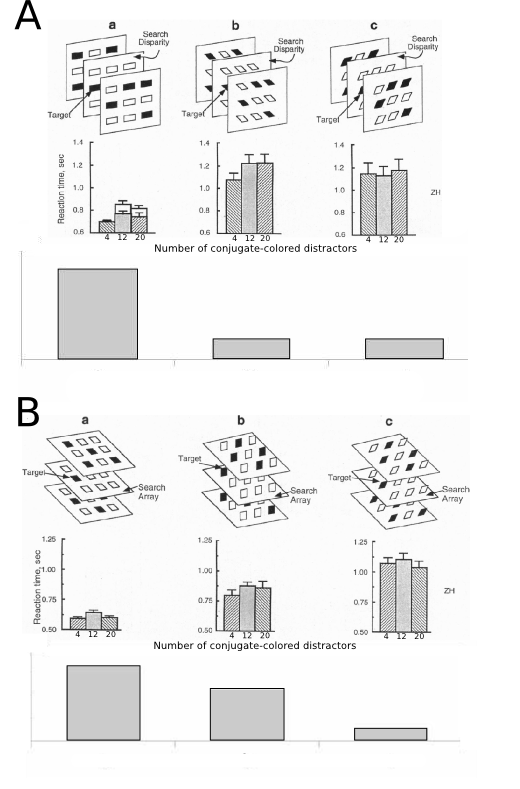
\includegraphics[width=3in]{3D-Surface/figs/nakayama}
\makeatletter
\let\@currsize\normalsize
\caption{Psychophysical and model results (adapted from ref~\cite{He_Nakayama95}). For each trial type (A or B), the top row shows the different stimuli, the middle row shows representative reaction times, and the bottom row shows the degree of attentional modulation of disparity-selective cells on the  attended plane. Increase in activity is assumed to be inversely proportion to reaction times.}
\label{ModelResults}
\end{figure}

\section{Results}
Figure~\ref{ModelResults} illustrates the experimental paradigm of He
and Nakayama \cite{He_Nakayama95}. In Figure~\ref{ModelResults}A, subjects had to search for the odd-colored target in the middle depth
plane; planes are outlined by rectangles that were not visible to the observers. The target was unique in this search plane but visually identical distractors  were present in other depth planes. In A-a, objects are aligned with the search plane while in A-b and A-c, they are slanted out of the plane. The middle row in A shows measured reaction times for three different numbers of distractors.They are significantly shorter when the objects are coplanar with the search plane (A-a) compared to when they are not aligned with the plane (A-b and A-c).

\begin{figure}[t]
\centering
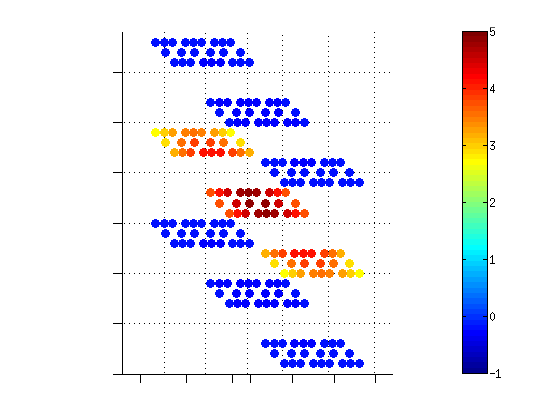
\includegraphics[width=3in]{3D-Surface/figs/attentionmod}
\makeatletter
\let\@currsize\normalsize
\caption{Spread of attention across surfaces. When attention is directed to the center slanted plane (as in the experiment in Figure 2B-a), attention enhances the activity of all cells along the surface (red), while suppressing the activity of cells belonging to other surfaces (blue).} 
\label{ModelResults2}
\end{figure}

In our model, we assume that the visual system can selectively direct
attention towards a specific surface by providing additional excitatory input to the grouping cell that represents this surface. As shown in Figure~\ref{NetworkStructure}, activity from the grouping cell selectively feeds back to all objects on that surface. In the case of Figure~\ref{ModelResults}A-a, the grouping cell corresponding to the middle fronto-parallel plane receives this attentional input. 
Activation of the disparity-selective cells in the search plane, shown in Figure~\ref{ModelResults}A-a, bottom row, is thus high. Among the objects in the search plane, the target has a unique color, which results in efficient search and the target being identified immediately. Reaction times are difficult to simulate in detail, therefore the increase in mean activity of disparity-selective cells on the attended plane due to attentional modulation is plotted instead,
which is assumed to be inversely proportional to reaction times. The
high activation level, bottom row, translates thus into short reaction
times, middle row.

In contrast, in Figure~\ref{ModelResults}A-b, the search plane is no longer a well-formed surface but contains objects that are slanted
backwards. Directing attention to the middle fronto-parallel plane
then has little effect on the disparity-selective cells in the search
plane. Search therefore cannot occur entirely within a single plane of coplanar, grouped elements and becomes inefficient, with much higher reaction times (middle row). These long reaction times are reflected in the low activation level of the disparity-selective cells (bottom row). Figure~\ref{ModelResults}A-c shows the analog result for figure elements that are slanted forward rather than backwards, as in A-b. Again, reaction times are long and population activity is low. 

The result is not restricted to fronto-parallel planes, as similar reaction time results were also found for slanted planes in Figure~\ref{ModelResults}B. When subjects are instructed to search in
a plane that is coplanar with the orientation of the figure elements
(middle plane in B-a), search is fast (B-a, middle row). In contrast,
when the figure elements do not align with the search plane (top row in B-b and B-c), reaction time is increased (middle row). Again, under the assumption that reaction times are inversely related to reaction times, the model reproduces human behavior (bottom row).

Attention to grouping neurons is then able to select sets of objects
organized in planes. Reaction times were fastest when the search array was a well-formed surface defined by locally coplanar elements. When search array elements were slanted away from this surface, reaction times increased. These results suggest that attention is linked to and spreads across perceived surfaces, which organize the visual scene
(Figure~\ref{ModelResults2}). 

\section{Surface Representation Using Basis Functions}
We investigated the use of basis functions to flexibly represent surfaces. Cite earlier studies using coordinate transforms

\section{Conclusion}
Using a simple model of perceptual organization in 3D,  we are able to reproduce psychophysical results from a visual search task that required allocation of selective attention to surfaces within the scene. The same grouping cells which organize the scene into planes also act as ``handles'' for top-down selective attention, enhancing the activity of coplanar elements belonging to the plane. Competition between grouping cells results in surface enhancement of the plane
corresponding to the attended grouping cell, and suppression of other
planes within the scene. Our proposed surface representation aids visual processing by providing a critical link between low-level
visual features and high-level object representations.